\documentclass[12pt, twoside]{book}

%\usepackage[margin=1.4in]{geometry}
\usepackage[utf8]{inputenc}
\usepackage{makeidx}
\usepackage[pass]{geometry}
\usepackage{fancyhdr}
\usepackage{xcolor}
\usepackage{graphicx}
\usepackage{url}
\usepackage{float}
\usepackage{verbatim}

\setlength{\marginparwidth}{0pt}
\setlength{\parindent}{0pt}
\setcounter{tocdepth}{3}

\newcommand\anotacion[1]{\Large\textcolor{red}{\\#1\\}\normalsize}
\newcommand\ant[1]{{\color{green}{#1}}}
\includeonly{summary,abstract,introduction,soa,tech,extensions,ccGadget,decisionMaker,videoConference,colorizer,results,discussion,conclusion,future,ref,append}

%\renewcommand{\chaptername}{}
%\renewcommand{\thechapter}{}

%% Style for the cover
\fancypagestyle{cover}
{
   \fancyhf{}
   \lfoot{
\includegraphics[keepaspectratio, scale=0.7]{Media/cc.png}}
   \renewcommand{\headrulewidth}{0pt}
}

%% Style for the pages with section
\fancypagestyle{sectioned}
{
   \fancyhf{}
   \rhead{}
   \renewcommand{\headrulewidth}{0pt}
}

\makeindex

\begin{document}

%% Front page
\pagestyle{fancy}
\renewcommand{\headrulewidth}{0pt}
\fancyhf{}
\cfoot{\fancyplain{}{\thepage}}
\lhead{}
\newgeometry{margin=2.5cm}
\begin{titlepage}
\pagenumbering{Roman}
\setcounter{page}{1}

\newpage
\thispagestyle{cover}
\begin{center}
  {\Huge \bf Framework de aplicaciones para red social colaborativa distribuida}

  \vfill
  {\LARGE\bf Pablo Martínez Bernardo}

  \vfill

  {\Large\bf Grado en Ingeniería Informática\\}
  {\Large\bf Facultad de Informática\\}
  \vspace*{0.2cm}
  {UNIVERSIDAD COMPLUTENSE DE MADRID}
  \vspace*{0.9cm}
  
   \begin{center}
   
\includegraphics[keepaspectratio, scale=0.12]{ucmlogo.png}
   \end{center}
  
  \vspace*{0.5cm}

  {\large\bf End-of-degree project\\
             Madrid, 1 de enero de 1970\\}
  \vspace*{0.7cm}
  {\large Director: Samer Hassan\\
          Co-director: Antonio Tenorio}

  \rhead{}
  \rfoot{}
  \fancyhf{}

\end{center}

\addtocontents{toc}{~\hfill\textbf{Page}\par}

%%%%%%%%%%%%%%%%%%%%%%%%%%%%%%%%%%%%%%%%%%%%%%%%%%%%%%%%%%%%%%%%%%%%%%%%%%%
%%%%%%%%%%%%%%%%%%%% Authorization of dissemination %%%%%%%%%%%%%%%%%%%%%%%  
%%%%%%%%%%%%%%%%%%%%%%%%%%%%%%%%%%%%%%%%%%%%%%%%%%%%%%%%%%%%%%%%%%%%%%%%%%%
\newpage
\thispagestyle{empty}
\addcontentsline{toc}{section}{\numberline{}Authorization of dissemination
                                            and usage}
\begin{center}
  \textbf{\Huge Authorization of dissemination and usage}
  \vfill
  {\Large Pablo Martínez Bernardo\\}
  \vspace*{1cm}
  {\Huge Signature goes here\\}
  \vspace*{1cm}
  {\Large Madrid, 1 de enero de 1970}
  \vfill
\end{center}

%%%%%%%%%%%%%%%%%%%%%%%%%%%%%%%%%%%%%%%%%%%%%%%%%%%%%%%%%%%%%%%%%%%%%%%%%%%
%%%%%%%%%%%%%%%%%%%%%%%%%%%% Acknowledgements %%%%%%%%%%%%%%%%%%%%%%%%%%%%%  
%%%%%%%%%%%%%%%%%%%%%%%%%%%%%%%%%%%%%%%%%%%%%%%%%%%%%%%%%%%%%%%%%%%%%%%%%%%
\newpage
\thispagestyle{empty}
\section*{Acknowledgements}
\addcontentsline{toc}{section}{\numberline{}Acknowledgements}

%%%%%%%%%%%%%%%%%%%%%%%%%%%%%%%%%%%%%%%%%%%%%%%%%%%%%%%%%%%%%%%%%%%%%%%%%%%
%%%%%%%%%%%%%%%%%%%%%%%%%%% Tables of contents %%%%%%%%%%%%%%%%%%%%%%%%%%%%
%%%%%%%%%%%%%%%%%%%%%%%%%%%%%%%%%%%%%%%%%%%%%%%%%%%%%%%%%%%%%%%%%%%%%%%%%%%
\newpage
\tableofcontents
\let\clearpage\relax
\newpage
\setcounter{page}{5}
\listoffigures
\listoftables
\newpage


%% Main text
% set page number starts from 1
\pagenumbering{arabic}

\newpage
\renewcommand{\thepage}{\Roman{page}}
\setcounter{page}{7}
\addcontentsline{toc}{section}{\numberline{}Abstract}
\section*{Abstract}
Apache Wave has been slowly developing since it was dropped by Google. Multiple aspects went away when that happened such as support, community and developers because some aspects remained undocumented, links were erased, and features truncated.\\[.2cm]
This work explores the scene of Wave, and specifically attemps to set the base for developers to code concurrent applications under the Wave infrastructure. Also, with the Robots API and Gadgets API, various open source and documented extensions have been created that solve some of the existing and unsolved needs in the current incarnations on Wave. It has also been in collaboration with other teams developing for Wave and has served the purpose of finishing and understanding incomplete documentation, which is a big impediment when trying to face development in Wave.\\[.2cm]
This can be the starting point for any developer interested in learning how to extend Apache Wave.
\vfill
{\large \bf Keywords:}\\
{\large Apache Wave, Collaboration, Gadgets, Robots, Wave Federation Protocol}


\pagestyle{fancy}
\renewcommand{\headrulewidth}{1pt}
%\renewcommand{\sectionmark}[1]{\markright{#1}}
\fancyhf{}
\rhead{\MakeUppercase{\leftmark}}
\cfoot{\fancyplain{}{\thepage}}
\lhead{}

\newpage
\thispagestyle{sectioned}
\pagenumbering{arabic}
\chapter{Introduction}
%\addcontentsline{toc}{chapter}{\thechapter{} Introduction}
Nowadays online social networks such as Facebook and Google+ are a big part of the mainstream Internet usage. There have been countless social networks in a very short span of time, and each time they are different and innovative, and are growing importance offline.\\[.2cm]
One of those remarkable attempts was \textbf{Google Wave}, that had a short life before Google dropped support and development, and even took the working nodes down. However the control was given to Apache to continue development of it. Since the inception of Wave, the web has undergone several changes, but the technology and protocol still remain relevant. JavaScript is one of the most used resources to execute code on the client-side\\[.2cm].
The world has also faced towards the cloud: applications are increasingly extracted from the personal computer and stored in a remote location to interact and share. One of the biggest advantages of the cloud is that it facilitates sharing, distributing creations among people. There is a similar concept to the one of sharing: \textbf{collaboration}, or being able to use the software simultaneously and in real time (Or almost real time) with other people and seeing the results. Wave embraced closely the concept of collaboration, and everything in it was geared towards it. Another successful Google collaborative product is Google Docs \cite{ref:google_docs} that predates Wave, as a consequence since then there have been other collaborative applications like Zoho \cite{ref:zoho}, Pads (Which are explained in Section \ref{subsec:color_soa}) and more.\\[.2cm]
With the growth of Facebook they began increasing the variety of features, and one of them that relates to this work is the arrival of Facebook Apps: applications developed by third parties but integrated inside Facebook by using some of its features.\\[.2cm]
When Google announced Wave it was an innovative product, and attracted positive attention. Google, disappointed with the adoption Wave received, and despite the enthusiasm from developers, stopped the development of Wave. They did not completely make it disappear, and instead chose to hand the project over to Apache to continue development, who deposited it on the Apache Incubator, a program for supporting promising open source software with the objective of converting it in an Apache Foundation project once it is mature enough.\\[.2cm]
Two of the important features of Wave since the beginning have been Robots and Gadgets: ways to \textbf{extend the capabilities of Wave} without the need to integrate them in the actual software, they can be made and changed independently. Gadgets are separate apps embedded inside another more powerful entity that hosts them. Robots interact with that same entity and are able to react to changes in it. The overall objective of this work is to create a framework around Wave, based on Gadgets and Robots, to explore their functionalities, help document their features and usage, and try to build a base so this two extensions can continue being explored and expanded in the future.\\[.2cm]
The P2Pvalue \cite{ref:p2pvalue} project has inspired the existence of this work and what is needed to be done. The P2Pvalue is a ``Techno-social platform for sustainable models and value generation in commons-based peer production in the Future Internet'', and are studying different aspects of social networks, and building an online collaboration platform on top of Wave to promote ``communities of collaborative production''.\\[.2cm]
The aim of this work is a framework, understood as the structure supporting a conglomerate of elements with a similar purpose or context. When Google dropped support for Wave, they also began sparingly removing web pages with very important information about it, and some of that information has been lost.

\section{Objectives}
This end-of-degree project was not intended to be just another exercise, but rather accomplish actual contributions to a real existing project. It then tries to put together every piece regarding gadgets and robots, test everything relating to them and lay a rough path so it can be followed in the future. This involves \textbf{documenting and testing} all the features provided by the available APIs.\\[.2cm]
However that is not the only intention, it was also important to make some tangible \textbf{extensions as robots and gadgets} that are useful for the Wave community, that satisfy needs not yet met. Everything has been open sourced and released under a free license \cite{ref:agpl} so it can be further improved and analyzed. The project P2Pvalue \cite{ref:p2pvalue} has been a great influence on what kind of features are needed, and some of them have been successfully accomplished.
\begin{itemize}
  \item {
    Wave Documentation
    \begin{itemize}
      \item Improve existing documentation
      \item Document undocumented features
    \end{itemize}
  }
  \item {
    Projects
    \begin{itemize}
      \item Updating existing projects
      \item Generating new useful extensions
    \end{itemize}
  }
  \item {
    Usage
    \begin{itemize}
      \item Explaining undocumented procedures
      \item Teaching how to start development of Wave extensions
    \end{itemize}
  }
\end{itemize}

\section{Document Structure}
All of those elements that compound the framework are explored individually. Those elements can be described individually, but the framework as a whole is also described. There are \textbf{global results and individual results}, and they are all organized as follows: first there is a global State of the Art and Methods, then each element is completely explained individually with its introduction, state of the art, results and conclusions, and finally global conclusions are reached. Also, every extension have their own results, conclusions and future work, but the complete work is analyzed as a single entity.\\[.2cm]
The objectives of the framework itself are the ones stated above, but every extension is also a whole project by themselves, so they have their specific objectives.
\begin{itemize}
  \item Chapter 3 - State of the Art: alternatives to Wave gadgets and robots.
  \item Chapter 4 - Technologies and methods: every procedure and technology that has been used along this work.
  \item Chapter 5 - Frame for Development of Gadgets \& Robots: how Gadgets and Robots work. How to get them running.
  \item Chapter 6 - CCWave: development of a Wave gadget for choosing a Creative Commons License.
  \item Chapter 7 - Pollymer: development of a Wave gadget for decision making.
  \item Chapter 8 - AppearWOW: development of a Wave gadget for video conference.
  \item Chapter 9 - Colbotia: development of a Wave robot for colorizing the contributions of each participant.
  \item Chapter 10 - Concluding Remarks: comments and analysis on the whole project.
\end{itemize}

\newpage
\thispagestyle{sectioned}
\chapter{Introducción}
%\addcontentsline{toc}{chapter}{\thechapter{} Introduction}
Hoy en día las redes sociales en línea tales como Facebook o Google+ son de gran importancia en el uso convencional de Internet. Numerosas redes sociales han surgido en un corto período de tiempo, han sido diferentes e innovativas, y disfrutan de una creciente importancia fuera de la red.
Uno de esos destacables intentos fue \textbf{Google Wave}, que tuvo una breve existencia antes de que Google decidiera dejar de dar soporte para él y desarrollarlo, e incluso desactivó los nodos que habían estado funcionando hasta entonces. El control del proyecto le fue otorgado a Apache para que continuara con su desarrollo. Desde el origen de Wave, la web ha sufrido numerosos cambios, pero la tecnología y el protocolo de Wave siguen hoy en día siendo relevantes. JavaScript es una de las tecnologías web más usadas hoy en día para ejecutar código en el cliente.
El mundo ha girado en el sentido de ``la nube'': las aplicaciones cada vez más son extraídas del ordenador del usuario y almacenadas en una localización remota para interactuar con ellas y compartirlas. Una de las principales ventajas de ``la nube'' es que facilita el intercambio entre usuarios, distribuir creaciones entre otras personas. Existe un concepto similar al de intercambio: \textbf{colaboración}, o usar aplicaciones de manera simultánea con otras personas y en tiempo real (O tiempo casi real) para ver el resultado a la vez. Wave siempre mantuvo cerca el concepto de colaboración, y todo en él estaba diseñado para colaborar. Otro exitoso producto de Google relacionado con la colaboración es Google Docs \cite{ref:google_docs}, que antedata a Wave, y por ellos desde entonces han existido otras aplicaciones colaborativas como Zoho \cite{ref:zoho}, Pads (Explicados en la Sección \ref{subsec:color_soa}) y otros.\\[.2cm]
Acompañando al crecimiento de la red social Facebook, desarrollaron varias nuevas utilidades, y una de ellas está muy relacionada con este trabajo y son las Apps Facebook: aplicaciones desarrolladas por terceros e integradas dentro de Facebook usando algunas de sus características.\\[.2cm]
Cuando Google anunció Wave fue una innovación, y atrajo una atención positiva. Google, decepcionados por una mala acogida del producto, a pesar de la buena aceptación por parte de los desarrolladores, decidieron ponerle fin al proyecto. No hicieron que desapareciera completamente, en su lugar eligieron otorgarle el proyecto a Apache con la intención de que continuara el desarrollo, y lo pusieron en el Apache Incubator, un programa para ayudar a prometedores proyectos de software libre con el objetivo de acabar incorporándolos como proyectos de la Apache Foundation cuando estén lo suficientemente maduros.\\[.2cm]
Dos de las características de Wave desde el principio han sido los Robots y los Gadgets: formas de \textbf{extender las capacidades de Wave} sin la necesidad de integrar nada en el software de Wave, así que pueden ser hechos y modificados de manera independiente. Los Gadgets son aplicaciones separadas pero empotradas dentro de una entidad más potente que ellos y que se encarga de contenerlos. Los Robots interactúan con esa misma entidad y pueden reacciónar a sus cambios y eventos. El objetivo general de este trabajo es crear un marco alrededor de Wave basado en Gadgets y Robots y así explorar sus funcionalidades, ayudar a documentar sus características y uso, además de cimientar una base para que estos dos tipos de extensiones puedan seguir siendo exploradas y mejoradas en un futuro.\\[.2cm]
El proyecto P2Pvalue \cite{ref:p2pvalue} ha inspirado tanto la existencia de este trabajo así como lo que era necesario hacer. P2Pvalue es una ``Plataforma tecno-social para modelos sostenibles y generación de valor en la producción de iguales basada en lo común en el Internet Futuro'', están estudiando diferentes aspectos de las redes sociales, y construyendo una plataforma online colaborativa basada en Wave para promover ``comunidades de producción colaborativa''.\\[.2cm]
El objectivo de este proyecto es un framework, entendido como la estructura que soporta un conglomerado de elementos con una intención o contexto similares. Cuando Google dejó de dar soporte para Wave, también empezaron lentamente a eliminar páginas web con información muy importante sobre Wave, y partes de esa información se han perdido.

\section{Objetivos}
Para este proyecto de fin de grado estaba pensado que no fuera simplemente un ejercicio más, sino llevar a cabo contribuciones reales a proyectos existentes. Por lo tanto se unen todas las piezas relacionadas con los Gadgets y Robots, se  prueba todo lo que tenga que ver con ellos y se dibuja un camino que podrá ser seguido más adelante. Para ello hay que \textbf{documentar y probar} todas las características que se ponen a nuestra disposición gracias a todas las APIs.\\[.2cm]
De todas maneras ésa no es la única intención, también es importante hacer algunas aportaciones tangibles en forma de \textbf{extensiones como Robots y Gadgets} que sean útiles para la comunidad de Wave, y que satisfagan necesidadas existentes que todavía no han sido solventadas. Todo el proceso se ha liberado en código y otorgado una licencia libre \cite{ref:agpl} para que otras personas puedan analizarlo y mejorarlo. El proyecto P2Pvalue \cite{ref:p2pvalue} ha sido una gran influencia en cuanto a qué características eran más necesitadas, y algunas de ellas han sido completadas satisfactoriamente.
\begin{itemize}
  \item {
    Documentación de Wave
    \begin{itemize}
      \item Mejorar documentación existente
      \item Documentar características no documentadas
    \end{itemize}
  }
  \item {
    Proyectos
    \begin{itemize}
      \item Actualizar proyectos ya existentes
      \item Generar nuevas extensiones útiles
    \end{itemize}
  }
  \item {
    Uso
    \begin{itemize}
      \item Explicar procedimientos no documentados
      \item Enseñar cómo introducirse al desarrollo de extensiones Wave
    \end{itemize}
  }
\end{itemize}

\section{Estructura del Documento}
Todos esos elementos que componen el framework serán explorados de manera individual. Pueden ser descritos individualmente, pero a su vez se puede describir el framework como unidad. Hay disponibles \textbf{resultados globales así como individuales}, y todos ellos están organizados de la siguiente manera: en primer lugar se encuentra un Estado del Arte general así como unos Métodos, y después cada elemento se explica completamente de manera indificual con su propia introducción, estado del arte, resultados y conclusiones. Finalmente se alcanzan unas conclusiones globales. Además de eso, cada extensión tiene sus propios resultados, conclusiones y trabajo futuro, pero el trabajo completo es analizado también como una entidad individual.\\[.2cm]
Los objetivos del framework en sí mismo son los descritos arriba, pero todas las extensiones son un proyecto completo en ellas mismas, por lo que tienen objetivos específicos.
\begin{itemize}
  \item Capítulo 3 - Estado del Arte: alternativas a los Robots y Gadgets de Wave.
  \item Capítulo 4 - Métodos y Tecnologías: cada procedimiento y tecnología que hayan sido usados a lo largo de este trabajo.
  \item Capítulo 5 - Marco para el Desarrollo de Gadgets y Robots: cómo funcionan los Gadgets y Robots. Cómo se pueden ejecutar.
  \item Capítulo 6 - CCWave: desarrollo de un gadget de Wave para elegir una licencia Creative Commons.
  \item Capítulo 7 - Pollymer: desarrollo de un gadget de Wave para toma de decisiones.
  \item Capítulo 8 - AppearWOW: desarrollo de un gadget de Wave para realizar vídeo conferencias.
  \item Capítulo 9 - Colbotia: desarrollo de un robot de Wave para colorear las contribuciones de los participantes.
  \item Capítulo 10 - Comentarios Conclusivos: comentarios y análisis del proyecto completo.
\end{itemize}

\newpage
\thispagestyle{sectioned}
\chapter{State of the Art}
%\addcontentsline{toc}{chapter}{State of the art}
This chapter will explore the global state of the art related to this work, and the evolution of gadgets and robots along the existence of the Internet.
\section{Generic Overview}
The concept of gadgets might have born with the name of apps in Google's ``Google Personalized Homepage'' in 2005 \cite{ref:what_happened_to_igoogle}, later to be called iGoogle (Figure \ref{fig:igoogle_2008}) and rename these components to gadgets. There is an important distinction to make: Nowadays hearing the words apps reminds us of portable phone applications. The word app insinuates smaller size and lesser complexity, and that is true for both kind of apps, but this work is exploring those \textbf{applications than run inside a bigger environment} and are embedded in it, extending it, but are not standalone and complete by themselves, they depend on the parent framework.
\begin{figure}[h]
  \center
    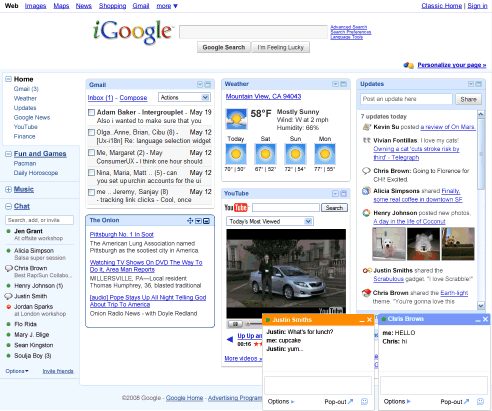
\includegraphics[keepaspectratio, scale=0.6]{Media/Captures/Soa/iGoogle.png}
  \caption{iGoogle in 2008}
  \label{fig:igoogle_2008}
\end{figure}
The social aspect of this apps was being able to share your gadgets with other people, and some examples of them would be weather apps, stock apps or video-watching apps.\\[.2cm]
In the latest years of iGoogle's life, before being discounted in 2012, iGoogle apps coexisted with Google Wave \cite{ref:wave_guide}, and Google Wave's Gadgets (Figure \ref{fig:wave_gadgets}). This other gadgets offered the advantage of the Federated Wave Protocol \cite{ref:wave_federation_protocol} and \textbf{real-time collaboration} \cite{ref:apache_wave_about}.\\[.2cm]
\begin{figure}[h]
  \center
    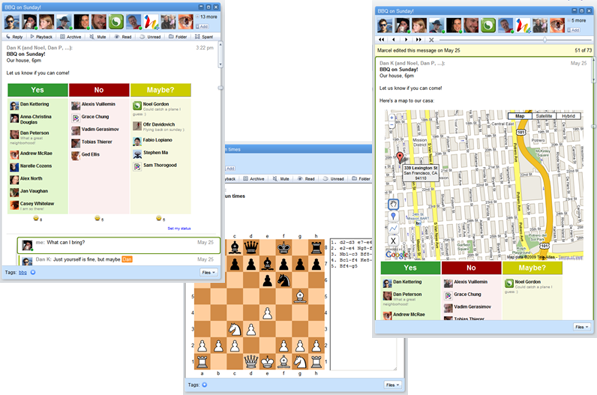
\includegraphics[keepaspectratio, scale=0.5]{Media/Captures/Soa/WaveGadgets.png}
  \caption{Google Wave Gadgets}
  \label{fig:wave_gadgets}
\end{figure}
Then Google began pushing Google+ \cite{ref:google_plus}, which can be considered to have some kind of gadgets in the shape of games, which were heavily influenced by Facebook games \cite{ref:facebook_games}, allowing users to play with other people from the same social networks, giving gifts and sharing scores.\\[.2cm]
Google also briefly had Spreadsheet Gadgets, which added unusual functionality for a spreadsheet application in Google Docs.\\[.2cm]
But Google has not been the only player in the world of applications. In the neat past Flash \cite{ref:adobe_flash} components have been omnipresent, basically for games but not limited for them. Another alternative for applications in the web are Java Applets \cite{ref:java_applets}, commonly use for scientific and learning purposes.\\[.2cm]
The other aspect explored in this work are robots, also known as bots. Robots usually interact loosely coupled from the software they are meant to interact with, but as with Wave Gadgets, robots can be incorporated in the main software, acting as an extension to it. An example of this are uNrEaL Bot \cite{ref:unreal_bot}, a collection of robots for very popular video games created to give the user an advantage over the rest of the players, integrating the graphical interface inside the game, and altering the game's own engine.\\[.2cm]
Robots are also \textbf{important in the web world itself}, but they are not usually productive bots, but instead robots made to emulate human behaviour to trick systems and people and get some kind of profit from it. It has been estimated that one third of the world's Internet traffic is made by automated robots \cite{ref:robots_in_the_web}. But this robots are different in the aspect that they are not meant to be: There's no intended resources for them and they take advantage of vulnerabilities, so as a result they can't run in harmony with the parent software, but as a parasite.

\section{Specifics}
As several extensions will been seen here, the specific state of the art relating each of them has been explored deeper in their specific chapters \ref{subsec:cc_soa}, \ref{subsec:decision_soa}, \ref{subsec:video_soa} and \ref{subsec:color_soa} respectively, so they are closer to their context.

\newpage
\section{Technologies}

\subsection{Wave}

In the making of this work every extension has been developed and tested under two varieties of Wave: Wave In A Box and Kune. Kune nowadays has much of it's code forked from the Wave In A Box repository, but adding more functionality around it. Gadgets and apps are built into the core of Wave, and as such Kune inherits all their capabilities, making gadgets and robots comparible with both technologies.\\[.2cm]
\begin{figure}[h]
  \center
    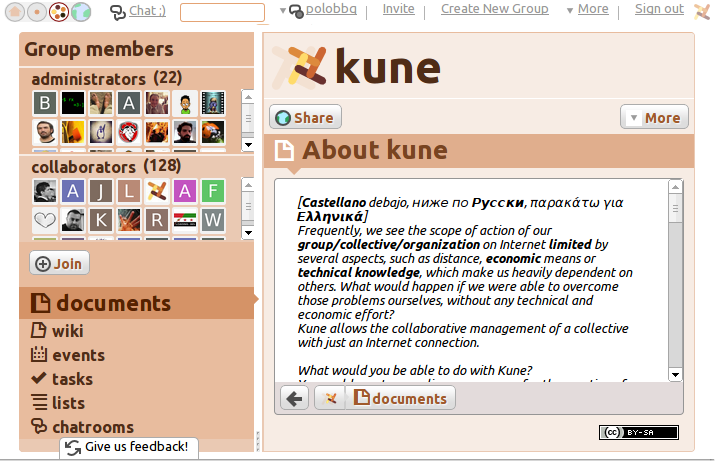
\includegraphics[keepaspectratio, scale=0.4]{Media/Captures/Wave/Kune_Groups.png}
  \caption{Kune Groups}
  \label{fig:kune_groups}
\end{figure}
The main technical feature that characterizes Wave is the Wave Federation Protocol \cite{ref:wave_federated_protocol}, that handles all of the communication happenning between users. It is an esxtension of the Extensible Messaging and Presence Protocol \cite{ref:xmpp}. Participants send delta changes on the content, and those deltas are distributed through the rest of the participants, guaranteeing that the end result is the same for everyone \cite{ref:federating_websites_google_wave}. Gadgets and robots will work under this environment, interacting with the Wave protocol.


\subsection{GWT}

Google Web Toolkit GWT is a set of tools that allows web developers to code in Java and from that java-compliant code, generate Asynchronous JavaScript and XML (AJAX) code to make front-end applications. The GWT framework focuses on efficiency and cross-browser compatibility, generating and then serving different AJAX code for every browser and locale combination, so the elements are rendered as they should in each browser, even though they behave differently. GWT provides the developer with all the common web controls, allows RPC invokations, browser history management, unit testing, and native JavaScript calls, among other features.\\[.2cm]
\begin{figure}[h]
  \center
    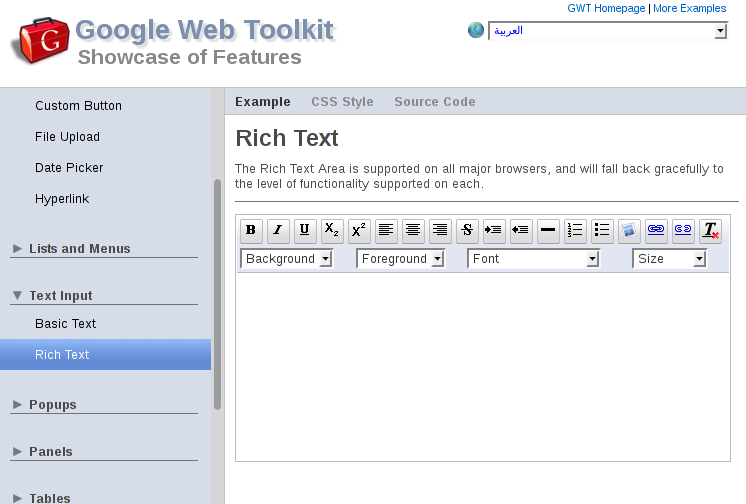
\includegraphics[keepaspectratio, scale=0.4]{Media/Captures/GWT/gwt_showcase.png}
  \caption{GWT Showcase}
  \label{fig:gwt_showcase}
\end{figure}
GWT has a development mode, where the Java code is not compiled to JavaScript, but instead it is ran in native Java and simulates the JavaScript components that will be used later. The development mode also allows a Java debugger to attach to GWT and debug the application locally. 


\subsection{Gadgets API}

The Gadgets API is made by Google to embed third party applications inside various Google products. They implemented it in wave as Wave Gadgets API, to have access to the specific features of Wave. These applications are HTML and JavaScript, with all their possibilities, and access specific features that the server can offer.\\[.3cm]
This is a Java API, and it needs to be compiled with the GWT compiler in order to be able to link to the gadgets. Apart from being able to use all GWT components, this API lets the developer communicate with Wave, and that means mainly altering the state and responding to state changes. The state contains the participants, and the content, among other information. 


\subsection{Robots API}

It is an API with client libraries for Java an Python, both of them implementing the same set of features. The original intention was that robots could act in Wave in exactly the same places and same ways as human participants could. In practice, not all interactions are implemented for robots. A robot can be added to a Wave, can edit text, add participants, publish new Wavelets, and access the contents of all of them, as well as responding to events about changes in the document or participants.


\subsection{Other}

\begin{itemize}
  \item As IDE Eclipse 3.8 has been used for developing the gadgets as well as the robot.
  \item OpenJDK has been used as JDK
  \item Jetty has been used for a local robot server
  \item Tomcat7 plus Shindig have been used as a local gadget server 
\end{itemize}


\begin{center}
------------------------------------------------------------------------------------------\\
\end{center}

\begin{itemize}
  \item Wave

  \begin{itemize}

    \item Wave can be interpreted as different things

    \item Protocol\\
    Google wanted a protocol to replace many aspects of online communication between people (mainly e-mail).\\
    Thus the Google Wave Federation Protocol exists. It is based on Extensible Message and Presence Protocol XMPP, which allows the secure communication of messages based on XML.\\
    The GWFP provides federation on top of XMPP, and it being an open protocol allows anyone to be a wave provider.
    
    \item Wave in a box\\
    Wave can also be used to refer to the software framework that allows users to communicate using GWFP.\\
    Originally called Google Wave, now Apache Wave or Wave in a box WIAB as the server implementation.

    \item Communication unit\\
    Inside WIAB, users are aggregated in what is called a Wave, there they can communicate and create different threads contained in that Wave.\\
    \anotacion{Include diagram showing the Wave(Wavelet(Blip(Document))) structure}    

  \end{itemize}

  \item GWT\\
  Google Web Toolkit GWT is a set of tools that allows web developers to code in Java and from that java-compliant code, generate Asynchronous JavaScript and XML AJAX to make front-end applications. The GWT framework focuses on efficiency and cross-browser compatibility, generating and then serving different AJAX code for every browser and locale to adjust the elements to fit properly.

  \item Gadgets API
  The Gadgets API is an API made by Google to embed third party applications inside various Google products. They implemented it in wave as Wave Gadgets API, to have access to the specific features of Wave. These applications are HTML and JavaScript, with all their possibilities, and access special specific features that the server can offer.

This is a Java API, and it needs to be compiled with the GWT compiler in order to be able to link to the gadgets. It has also a development mode, wich runs native Java and recreates the components without needing a web server.

  \item Robots API
  It is an API with client libraries for Java an Python, both of them with a similar syntax.\\
  The original intention was that robots could act in Wave in exactly the same places and same ways as human participants could. In practice, not all interactions are implemented for robots.\\
  A robot can be added to a Wave, can edit text, add participants, publish new Wavelets, and access the contents of all of them.
\end {itemize}

\begin{itemize}
\item \anotacion{What other things should I talk about?}
\item \anotacion{``Materials'' doesn't make sense, ``Methods'' does. This includes a (technical) explanation/description of the technologies used. You can mention the challenges implied by the lack of documentation, as Google didn't release all the software/docs/APIs/etc. The specific problems go in Results/Discussion, not here, as here the approach is ``before'' implementation.}
  \item Wanted to explore both ways to extend wave
  \item Talk about specific software I used?
  \item How to create a gadget, alternatives, GWT (How is GWT used in wave, what does GWT do)
  \item How to create a robot, alternatives, how much detail?
  \item Servers for gadgets and robots, how to communicate them with wave
  \item Should I talk about the problems I had?
  \item Talk about the lack of documentation?
\end{itemize}

\newpage
\section{Extensions}

Both possible ways for extending Wave have been explored in this work. Gadgets have been implemented with the Wave Gadgets API, and robots with the Java version of the robots API.

Wave gadgets live inside a wave, and therefore are able to interact with it. Among other things, they can access the current state of the wave. There is two different kinds of state:

\begin{itemize}
  \item Private State\\
        Stores information that can only be accessed from the participant that modified it.
  \item Shared State\\
        Stores the global state of every gadget in this wave.
\end{itemize}

The state is actually an entity containing key-value pairs of strings. The state can be modified at any time, and the changes made to it will be communicated to the rest of the participants, so they can react accordingly to this change. This is represented in the next figure:

\anotacion{TODO: Explain the diagrams a little}

\begin{center}
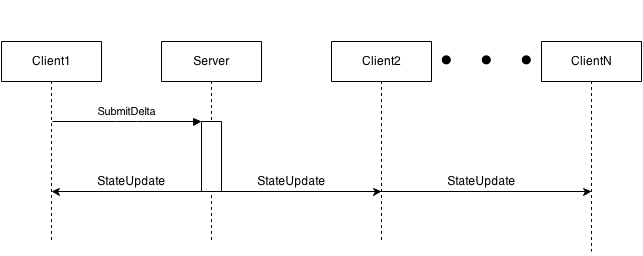
\includegraphics[keepaspectratio, scale=0.6]{Media/Diagrams/State/StateSequence.png}
\end{center}


The Gadgets API requires you to create a class hierarchy to be able to succesfully compile. In a hypothetical gadget named ``Gadget'' it would be as follows:

\begin{center}
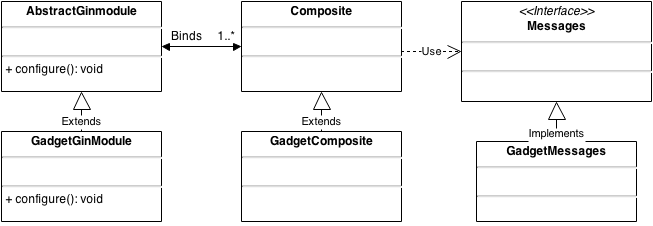
\includegraphics[keepaspectratio, scale=0.5]{Media/Diagrams/Gadget/Gadget.png}
\end{center}

For every gadget project it has also been implemented a tester and a deployer.

The intention of the tester is to take advantage of the ``Development Mode'' in GWT that allows you to run the code locally without deploying it to a web server. The class diagram for every tester project has followed the same pattern:

\begin{center}
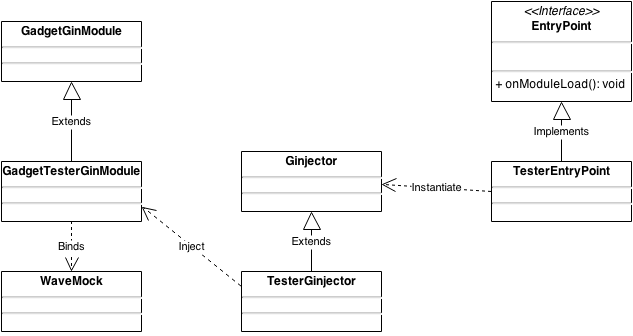
\includegraphics[keepaspectratio, scale=0.6]{Media/Diagrams/Gadget/Tester.png}
\end{center}

The project is then run as a Web Application with Google's App Engine.

The deployer also follows a similar pattern:

\begin{center}
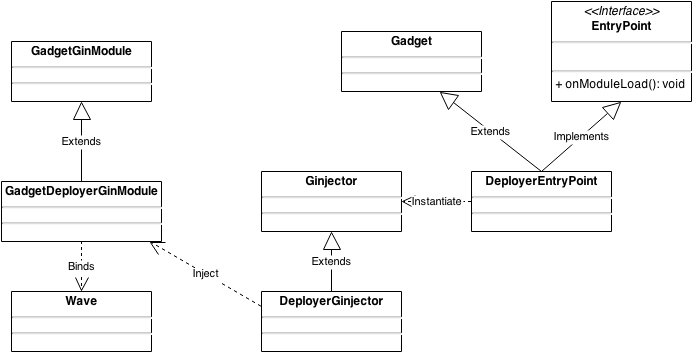
\includegraphics[keepaspectratio, scale=0.5]{Media/Diagrams/Gadget/Deployer.png}
\end{center}

The difference between this two structures are the following: First, a Wave Mock is no longer needed, as our gadget will be in an environment with a real Wave behaviour, so the Wave class is bound from the GinModule. Also, the entry point now also extends the Gadget class, a class given by the Gadgets API which some behaviour needed for the Gadget to work in an actual environment.

\subsection{Creative Commons Gadget}

\subsubsection{Introduction}
The default license for any creation of any kind is the restrictive copyright. Copyright tries to ensure that all the rights remain to the original author of the content, but sometimes it can be advantageous to let people freely or semi-freely use, distribute or modify the content. One of the most popular, with over 400 million \cite{ref:the_power_of_open}, are the Creative Commons set of licenses. These are not adecuate for licensing software, but in the context of Wave the content is usually creative work, for which Creative Commons makes a good job.

\subsubsection{State of the Art}
Wave doesnt have any way of publishing your content under any specific license. Kune has the option for publishing Waves in your personal space under one of the existing Creative Commons Licenses. Outside of the personal space, Kune preserves Wave's aspect and removes the space where the license is in the personal space, so no license is imposed to other participants in a wave.

\subsubsection{Results}
This extension allows participants to set a Creative Commons license to a specific blip, by inserting a gadget in the content and answering questions to reach the adequate license that meets the requierements. The Figure \ref{fig:cc_gadget} shows the final result of this extension.

\begin{figure}[h]
  \center
    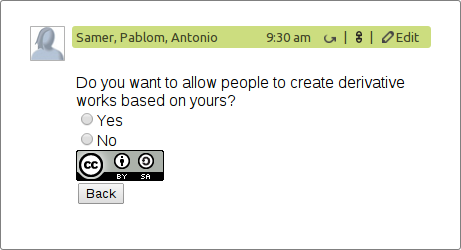
\includegraphics[keepaspectratio, scale=0.7]{Media/Captures/Extensions/CCGadget.png}
  \caption{Creative Commons Gadget}
  \label{fig:cc_gadget}
\end{figure}


\thispagestyle{sectioned}
\chapter{Pollymer}
%\addcontentsline{toc}{chapter}{\numberline{Decision Maker Gadget}}
When talking in a group of people it is sometimes necessary to take a decision about a specific aspect. The easiest way to achieve this is by talking, and Wave with real time communication and editing common documents makes this easy. But this way it might be difficult to easily differentiate all the different options, see who agrees with each one of the options, or quickly decide one. This extension allows every participant to \textbf{choose an option or add new options to the decision}. Participants are also able to quickly see who voted each option along with their user avatar images. This features accompanied by Wave's style of communication make consensus and decision making easier.

\label{subsec:decision_soa}
\section{State of the Art}
Because of the nature of Wave, decision making is a very important and basic, so there has been several gadgets made regarding that. It also easily explores all the basic possibilities that the Gadgets API provides. Figures \ref{fig:poll} and \ref{fig:consensuall} show two of them: The first one is Poll by Eric Williams, focused on showing statistics about the results, maybe useful when there is a high amount of votes. The second one is Consensuall \cite{ref:consensuall} by Antonio Tenorio, focused on sharing the personal opinion of each voter about an issue and reaching consensus on it.\\[.2cm]
\begin{figure}[h]
  \center
    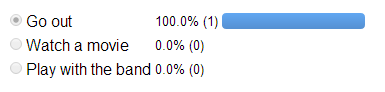
\includegraphics[keepaspectratio, scale=0.7]{Media/Captures/Extensions/DecisionGadgets/other.png}
  \caption{Poll}
  \label{fig:poll}
\end{figure}
\begin{figure}[h]
  \center    
    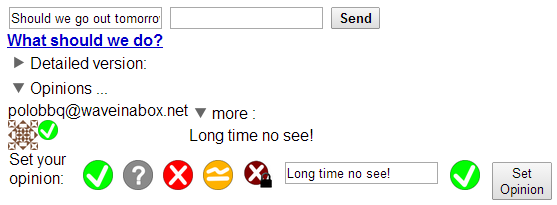
\includegraphics[keepaspectratio, scale=0.7]{Media/Captures/Extensions/DecisionGadgets/consensuall.png}
  \caption{Consensuall}
  \label{fig:consensuall}
\end{figure}
Pollymer falls in between both of them by letting people add their own answers, see a representation of the votes and who personally voted for each.

\section{Results}
Pollymer is a gadget that can be inserted anywhere in a blip. A title is chosen for the issue at hand, and then \textbf{different options} answering that title can be inserted by anyone who sees the gadget, not only the creator. One of the decisions can be instantly chosen by clicking on it.
\begin{figure}[h]
  \center
    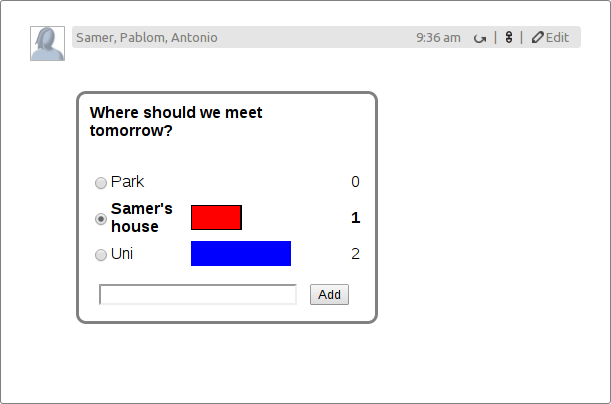
\includegraphics[keepaspectratio, scale=0.35]{Media/Captures/Extensions/DecisionMakerGadget.png}
  \caption{Pollymer}
  \label{fig:decision_maker_gadget}
\end{figure}
When there have been decisions chosen by different participants, \textbf{hovering the mouse over} the number of votes on the right will show the names and pictures of the participants that voted for it, as represented in Figure \ref{fig:decision_maker_votes}. Names and pictures are taken from their Wave profile.
\begin{figure}[h]
  \center
    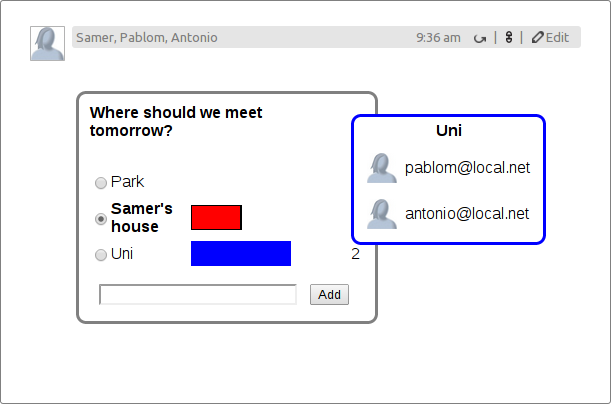
\includegraphics[keepaspectratio, scale=0.35]{Media/Captures/Extensions/DecisionMakerGadget_votes.png}
  \caption{Pollymer Voters}
  \label{fig:decision_maker_votes}
\end{figure}
This gadget also relates to the structure shown in Figure \ref{fig:gadget_classes}. The GinModule is the DecisionMakerGinModule, the Composite is the DecisionMakerMainPanel, and the Messages class is represented by the class DecisionMakerMessages. This gadget is slightly more complex than the Creative Commons one, so the class diagram with its specifics is shown in Figure \ref{fig:decision_maker_diagram}.
\begin{figure}[h]
  \center
    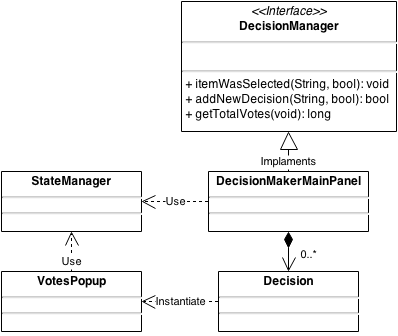
\includegraphics[keepaspectratio, scale=0.5]{Media/Diagrams/Gadget/DecisionMaker.png}
  \caption{UML Class Diagram, Pollymer}
  \label{fig:decision_maker_diagram}
\end{figure}
The interface DecisionManager is extended. It is meant to represent all that can be done with the decisions: select one, add a new decision, and get the total votes of one specific decision. The DecisionMakerMainPanel implements it, and is also the container for all the decisions. A decision represents one of the options that can be chosen, and generates the Popup showing who voted for it. A StateManager is also used to handle everything related to the Wave's state.\\[.2cm]
There are three different types of entries in the Wave's state:
\begin{itemize}
  \item \textbf{Count of votes}: There is one entry of this kind for each decision. To identify which decision this entry is for, the title of the decision is stored as a key. Therefore, the decision titles have to be unique. The value of this entry is the amount of votes that decision has, making it quick to retrieve the amount and show the vote count.
  \item \textbf{Voters}: Again, one entry for each decision and the title of the decision as an unique identifier. The value is a list of all the people that voted for that decision. As the state is only able to store a string, the list is like \verb+|user1@kune.cc|user2@kune.cc|user3@kune.cc|+. This entry is used to know if a particular user has voted for a decision, and to fill the information inside the votes popup.
  \item \textbf{Title}: There is one single entry for each gadget. The value of this entry is the name of the decision to be taken. Used to fill the title after it has been set.
\end{itemize}
\section{Conclusions and Future Work}
There are already several alternatives for decision making, each one with their unique way of doing things, and there is certainly already one suitable for every need, and Pollymer doesn't innovate in almost any aspect. This alternative has limitations though: There is no option for multi-choice answers, no way of editing the title after being created, and the list of votes can get a little uncomfortable to see after a large amount of votes has been made. Multi-choice answers would put this gadget \textbf{closer to a consensus tool}, and being able to block options would make the divergence among opinions more visible.
\newpage

\thispagestyle{sectioned}
\chapter{AppearWOW}
\label{subsec:video_intro}
%\addcontentsline{toc}{chapter}{\numberline{Video Conference Gadget}}
From D1.3 Design Guidelines (Section Technical Features) \cite{ref:p2pvalue}: ``The platform should therefore include tools for collaboration, including key features, such as: Synchronous communication with video and voice communication''.\\[.2cm]
Wave is meant for text communication. Text has the advantage that it can be stored easily, searched later and edited simultaneously, but lacks the naturality of human-to-human interaction. To get as close as possible to it we need voice and video. Then collaborating on text can be made more efficiently. This gadget makes it possible to \textbf{speak to up to 16 other users and see them}.

\section{State of the Art}
\label{subsec:video_soa}
There is no alternative to video or audio communication integrated on Wave. There is other alternatives though outside of it, some of them shown in Figure \ref{fig:skype_hangouts}.
\begin{figure}[h]
  \center
    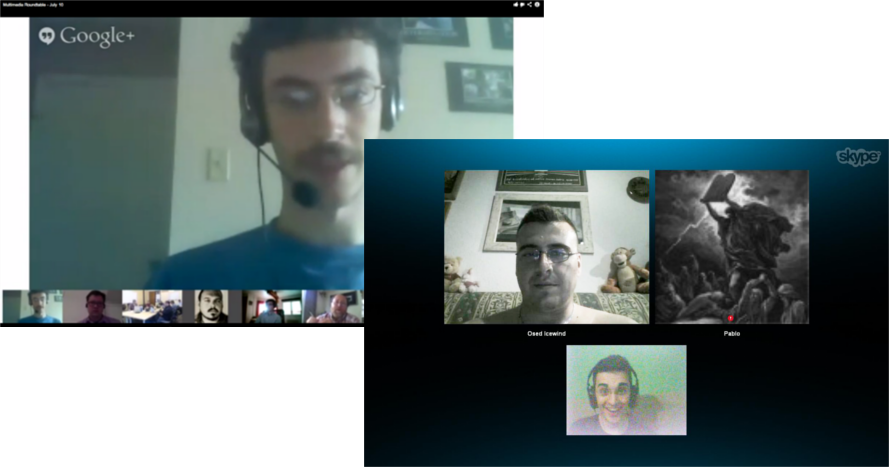
\includegraphics[keepaspectratio, scale=0.43]{Media/Captures/Soa/skype_hangouts.png}
  \caption{Hangouts and Skype}
  \label{fig:skype_hangouts}
\end{figure}
They focus on video, even hiding text communication to leave more room to the video. AppearWOW can be mixed with text above and below, leaving the video communication as an addition and not the main point. Both video communication tools shown (Google's Hangouts and Microsoft's Skype) require you to have a specific user account to use their services, while this gadget lets you join the \textbf{video communication from within Wave}, but also from an external link without giving any kind of personal information.

\section{Results}
To make this gadget it has been essential the use of a pre-existing service called \textbf{appear.in} \cite{ref:appearin}. They provide the whole video and audio communication based on WebRTC \cite{ref:webrtc}, and also facilitate an easy way to use their service in an external website. It is a JavaScript component that can be put inside an iframe, and it will take care of almost everything. Figure \ref{fig:video_gadget} shows the final result of this integration.
\begin{figure}[h]
  \center
    
\includegraphics[keepaspectratio, scale=0.8]{Media/Captures/Extensions/VideoGadget/RoomSelection.png}
  \caption{Room Selection Screen}
  \label{fig:video_gadget_room}
\end{figure}
When a user inserts the gadget, he will be prompted with the room selection screen shown in Figure \ref{fig:video_gadget_room}, letting him choose the identifier of the room people will meet in. The same room can be visited from different waves, and also directly from appear.in, as room names can not be duplicated.
\begin{figure}[h]
  \center
    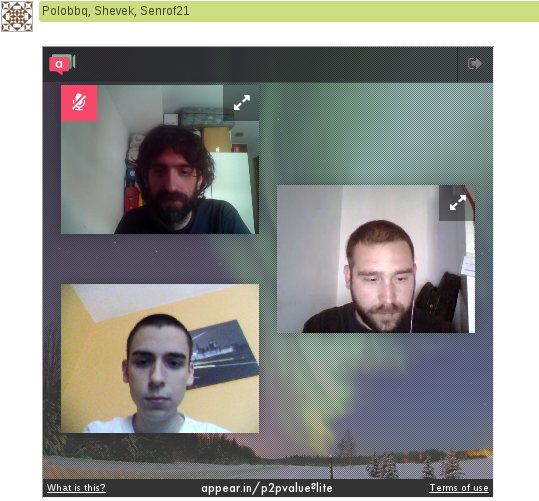
\includegraphics[keepaspectratio, scale=0.45]{Media/Captures/Extensions/VideoGadget.png}
  \caption{Video Conference Gadget}
  \label{fig:video_gadget}
\end{figure}
It was shown in Figure \ref{fig:gadget_classes} the basic structure of a gadget. The composite is represented by the VideoGadgetMainPanel, the Messages are the class VideoGadgetMessages, and the GinModule is realized by VideoGadgetGinModule. Outside from that, the structure is relatively simple.\\[.2cm]
As appar.in is a JavaScript service, multiple calls to \textbf{native JavaScript} have been made inside this gadget.
The service appear.in uses the name of the room as a unique identifier, so the gadget asks the user for a name before entering the room. The gadget also makes use of appear.in's \verb|?lite| feature, that simplifies the user interface, leaving more space for the images of the video. The \textbf{camera is accessed through the browser}, so no additional software has to be installed.\\[.2cm]
The Wave state in this gadget is really simple, the only thing stored in it is the name of the room to enter it directly if it has already been set.\\[.2cm]
\begin{figure}[h]
  \center
    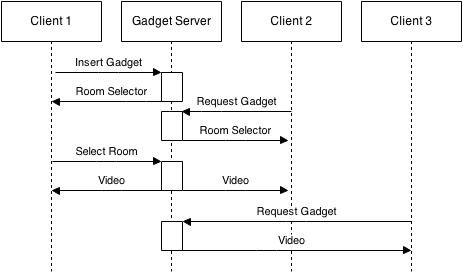
\includegraphics[keepaspectratio, scale=0.6]{Media/Diagrams/Gadget/VideoSequence.png}
  \caption{UML Sequence Diagram, AppearWOW}
  \label{fig:video_gadget_sequence}
\end{figure}
Figure \ref{fig:video_gadget_sequence} shows how the gadget reacts to requests. Once the gadget is inserted, the room selection screen will be shown, allowing any participant to select the name of the room the participants will meet in. When a room is selected, the participants automatically enter the room. If another participant joins the wave once the room has been selected, he will be served the video conference directly.
\section{Conclusions and Future Work}
The fact that this extension is completely \textbf{dependant on an external closed-source service} is a big limitation. The service could stop working at any time, technical improvements on video or audio communication can not be made, limitations like the maximum of 16 online users can not be avoided, the way to use it could change making it necessary to update the gadget, and other changes may arise.
\newpage

Robots were created in Wave with the intention to be able to act exactly as an actual human participant. Revisiting Figure \ref{fig:wave_structure} we can understand how robots can participate: They are invited to the Wave by inserting their unique identifier. They will aprear as invited without any apparent indication that they are a robot. Robots can make changes to the Wave such as creating a new blip, editing them, changing annotations...\\[.2cm]
In order to be able to interact with Wave it is necessary to register the robot with the Wave server where the robot will be run. For example, for the Kune node kune.cc, go to \url{http://kune.cc/robot/register/create} and you will be prompted with the screen shown in Figure \ref{fig:robot_register}.
\begin{figure}[H]
  \center
    
\includegraphics[keepaspectratio, scale=0.6]{Media/Captures/Wave/RegisterRobot.png}
  \caption{Robot Registration Screen}
  \label{fig:robot_register}
\end{figure}
As username set the name you wish to give your robot, it should be a free name in the server, as names are unique. In the URL enter the URL where the gadget will be launched, it should be an URL reachable from within the Wave server. After sending the data you will receive a Consumer Token matching the name you entered, and a Consumer Token Secret: a secret key you will need to use to authenticate with OAuth and guarantee the identity of your robot.\\[.2cm]
There is no equivalent to the tester mode from GWT, but running a server for the robots is easy enough so it is not a hassle. Using Maven plus Jetty you can set the Maven goal to \verb|jetty:run| and the robot will be run.\\[.2cm]
Robots do basically two thins: Act when needed, and react to events. Acting means modifying the documents, creating new blips... And receiving events means a callback will be made to the robot when something from an external action happens on the Wave. The kind of events that are notified to the robot are the following:
\begin{itemize}
  \item WaveletBlipCreated: Triggered when a new blip is created.
  \item WaveletBlipRemoved: Triggered when a blip is deleted.
  \item WaveletParticipantsChanged: Triggered when a participant is added or removed.
  \item WaveletSelfAdded: Triggered when the own robot is added as a participant.
  \item WaveletSelfRemoved: Triggered when the own robot is removed as a participant.
  \item DocumentChanged: Triggered when the text of a document changes.
  \item AnnotatedTextChanged: Triggered when the annotations of a document change.
\end{itemize}
There are other events documented such as GadgetStateChanged or WaveletTagsChanged, which even though available through the Robots API will not be triggered on the server, and therefore never received.

\subsection{Colorizer Robot}
Again, text communications gets in the way of collaboration in some aspects. When working between several people it is sometimes necessary to talk about some aspect of the work they disagree in. In plain text, when there are more than two collaborators, there is no way to know who edited what, so those kind of issues can't be addressed personally. A robot is needed in order to know when and what changes are being made.

\subsubsection{State of the Art}
In Wave it is possible to see who has participated in a blip as shown in Figure \ref{fig:participants}, but it is not possible to see exactly what that participant has modified what part of the document.
\begin{figure}[H]
  \center
    
\includegraphics[keepaspectratio, scale=0.7]{Media/Captures/Wave/Participants.png}
  \caption{Blip Participants in Kune}
  \label{fig:participants}
\end{figure}
The other thing Wave does to try to keep people informed on when changes happen, is to highlight the changes that just happened and write the author's name next to it, as shown in Figure \ref{fig:participants2}. The problem is it is not permanent, so you only realize of the change if you were already looking at the content being changed.
\begin{figure}[H]
  \center
    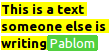
\includegraphics[keepaspectratio, scale=0.7]{Media/Captures/Wave/Participants2.png}
  \caption{Change Highlighting in Kune}
  \label{fig:participants2}
\end{figure}
Also, this extension is heavily inspired in Pads, services like PiratePad, Etherpad, TitanPad and many others, that offer an online collaboration tool that allows to concurrently write plain-text documents. They show a specific color for each participant to quickly see who edited what. TitanPad in Figure \ref{fig:titanpad}, even though not the only, has the capability to show a timeline and revisit past states of the Pad, so no information is lost even after being modified.
\begin{figure}[h]
  \center
    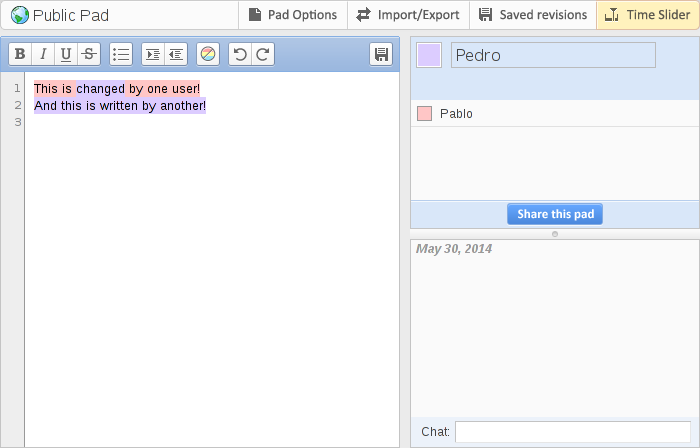
\includegraphics[keepaspectratio, scale=0.4]{Media/Captures/Soa/TitanPad.png}
  \caption{TitanPad}
  \label{fig:titanpad}
\end{figure}

\subsubsection{Results}
This extension, in the shape of a robot, goes around that problem by assigning a color to each participant, and painting the background of the text that participant edits. The result can be seen in Figure \ref{fig:colorizer_editions}. It also keeps track of who has each color and puts it in a blip under the main blip of the wave, as seen in Figure \ref{fig:colorizer_editors}. It is also possible to get around the colorizing of any given blip by starting it with \verb|@Robot clear annotations|, being ``Robot'' the actual name of the robot that it was registered with.\\[.2cm]
\begin{figure}[H]
  \center
    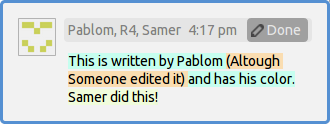
\includegraphics[keepaspectratio, scale=0.8]{Media/Captures/Extensions/Colorizer/ColorizerEditions.png}
  \caption{Colorizer Robot Colors}
  \label{fig:colorizer_editions}
\end{figure}
\begin{figure}[h]
  \center
    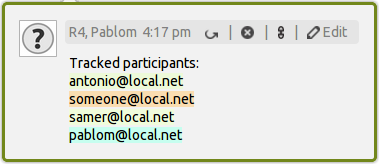
\includegraphics[keepaspectratio, scale=0.7]{Media/Captures/Extensions/Colorizer/ColorizerEditors.png}
  \caption{Colorizer Robot Tracking Participants}
  \label{fig:colorizer_editors}
\end{figure}
The way to make the background of the text be of a specific color is by changing the annotations of the document. Annotations in Wave are tags affecting a range of text and altering its properties, but they don't affect the text itself. Annotations are also able to be transmitted through the Federation Protocol. Every annotation is defined by a name (What it does), a range (What characters of text it affects), and a value (What value should that annotation take on that range). There are annotations for text size, links, language... For this robot specifically the annotation \verb|style/backgroundColor| is the one being set in the changed text.\\[.2cm]
The way to know when the changes happen is by subscribing th the DocumentChanged event explained before. This event will be triggered anytime anyone modifies the text.\\[.2cm]
\begin{figure}[h]
  \center
    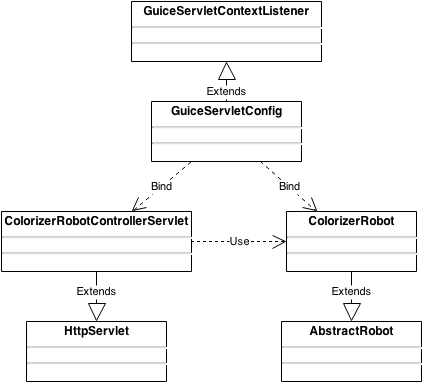
\includegraphics[keepaspectratio, scale=0.5]{Media/Diagrams/Robot/Colorizer.png}
  \caption{Colorizer Robot Class Diagram}
  \label{fig:colorizer_diagram}
\end{figure}
That only leaves one task left: The DocumentChanged event tells us the document has changed, but not what part changed or how it changed, so it is up to us to extract that information. To achieve it Google's google-diff-match-patch, a Java library that is able to extract the difference between two chunks of plain text. Every time the document is changed, the difference with the last version is calculated, and the new content is attributed to the participant that changed it.\\[.2cm]
Figure \ref{fig:colorizer_diagram} represents the class structure of the Colorizer Robot. The HttpServlet is the responsible of receiving the communication from the Wave Protocol. The ColorizerRobot sets up the OAuth authentication with the token received when registering the robot. Also, thanks to the AbstractGadget class it is registered to receive all the events. The GuiceServletConfig binds the necessary dependencies together.\\[.2cm]
This extension, as said before, uses an API for diff that works with plain text. That means changes on annotations are not detected. Also, diff detection can be problematic in some cases. The difference between two documents is always computed correctly, but as the library does not have information on where the text changed, it will sometimes attribute a change to a wrong position of the text. For example: We have the string ``abc'', and a participant decides to add a new ``b'' to the left of the already existing ``b''. The end result would be ``abbc'', where the first apparition of the letter will be the change from the last version of the text. But because of how the diff calculation is made, the library will come up with the result that the difference between those two texts is the ``b'' on the right and the robot will put the background color in the wrong character. This small example can be extrapolated to more complex and problematic cases.


\anotacion{Talk about how gadgets and robots can be run (tomcat, shindig, jetty)}

\anotacion{Talk about documentation}

\chapter{Concluding Remarks}
The whole end-of-degree project is analyzed in the following sections regarding the results of the work, the conclusion reached after its development, and future lines of work that could be followed after making this work.
\section{Discussion of Overall Results}
%\addcontentsline{toc}{chapter}{\numberline{Global Results}}
Developing for Wave is \textbf{full of difficulties}. When Google released the project to the Apache Foundation to put into the Incubator they didn't fully release everything, keeping parts of the software hidden. There was lack of documentation for many features, and over time links with important information about Wave have been deleted without replacement. This informality leaves the developer with the only option of trial and error to make things work.\\[.2cm]
Many of these extensions, specifically the Creative Commons License Gadget, the Colorizer Robot and the Video Conference Gadget, or better said the base concepts behind them, had already been suggested for the P2Pvalue project to build, so they meet actual needs that the Wave community has right now.\\[.2cm]
There are attemps to \textbf{increase the accessibility to Wave} not only to users, but also to developers. That means improving visibility of all the projects related to Wave, completing the features that Wave is lacking right now, and documenting important things that act as tall walls for a developer that wants to get into it. This end-of-degree project contributed to review documentation about Wave gadgets and robots and add to it, as well as updating the sample gadget provided in the Kune repository to one working for the latest version of Kune and a newer version of the GWT.\\[.2cm]
It would have been useful to make a \textbf{bigger framework}, with more variety and amount of gadgets. Suggested future work in the previous chapters is sometimes outside of the purpose of a framework for gadgets and robots, but the application framework itself can also be improved: Because of the increased difficulty in getting into the development there are procedures that were intended to be documented but haven't been. Also, this work is only as useful as the people who see it, then it will benefit from being spread.\\[.2cm]
The reasons for developing each of the extensions, as well as the contributions to documentation have been explained in the capter for each extension, but Table \ref{fig:contributions} shows them summarized.
\begin{table}[h]
  \footnotesize
  \begin{center}
    \begin{tabular}{ | l | p{2.49cm} | p{2.1cm} | p{2.2cm} | p{2.3cm} |}
      \hline
      \textbf{Extension} & \textbf{Need Satisfied} & \textbf{Features} & \textbf{Interacts With} & \textbf{Contributions}\\
      \hline
      \ref{subsec:cc_intro} - CCWave & D1.3 Design Guidelines (Section Legal Regime) \cite{ref:p2pvalue} & Choose a Creative Commons License for the content of a blip & Gadgets API & Gadget Development Tutorial \cite{ref:gadget_development}\\
      \hline
      \ref{subsec:decision_intro} - Pollymer & & Poll users about a question & Gadgets API & Gadget Development Tutorial \cite{ref:gadget_development}\\
      \hline
      \ref{subsec:video_intro} - AppearWOW & D1.3 Design Guidelines (Section Technical Features) \cite{ref:p2pvalue} & Video conference communication & Gadgets API, appear.in & \\
      \hline
      \ref{subsec:color_intro} - Colbotia & D1.3 Design Guidelines (Section Economic Model) \cite{ref:p2pvalue} & Highlight the contributions of each participant & Robots API, OAuth & Development Tutorial \cite{ref:robot_development}, Sample README \cite{ref:readme_sample}, Registration Process \cite{ref:registration_process}\\
      \hline
    \end{tabular}
  \end{center}
  \caption{Contributions to Documentation}
  \label{fig:contributions}
\end{table}


\section{Conclusion}
%\addcontentsline{toc}{chapter}{\numberline{Conclusion}}
Gadgets by nature are just embedded interactuable applications, slightly decoupled from the context they are in. With increasing computing power, even in mobile devices, the big difference \cite{ref:javascript_slow} in power needed to complete a task between JavaScript and other native languages starts getting neglegible. GWT achieves \textbf{high compatibility} with all different browsers, and with the help of different APIs can be a very good tool for creating gadgets in situations where the concept of the gadget makes sense. The only limitation is it is not possible to get outside of the gadget apart from what the API provides.\\[.2cm]
Gadgets are a relatively \textbf{easy way to extend Wave}, as no actual knowledge of Wave's codebase is needed to do so. But still the Gadgets API is far from perfect, and requires the developer to repeat tasks for every gadget made. Also, there will be sometimes version compatibility problems, project configuration problems, classpath errors, and the messages given by the GWT compiler are not informative enough. Many steps need to be followed to get things working.\\[.2cm]
Also, even though the Gadgets API is a Java API, the fact that it generates JavaScript code means troubleshooting is sometimes needed in the JavaScript layer, so JavaScript knowledge is also needed, and computer generated code can sometimes not be easy to follow and understand.\\[.2cm]
The wishes by which this work was inspired have definitely been satisfied.\\[.2cm]
As a framework, succesful development of both gadgets and robots has been carried out completely from start to finish, using \textbf{all the important and interesting features} provided by the Gadgets API and Robots API. Not only that, but also issues have been documented and samples have been provided to the public to use.\\[.2cm]
Useful gadgets have also been developed. They were inspired by \textbf{actual needs}, and have been finished to a ready to use state. Anyway, they are openly available under the Affero General Public License\cite{ref:agpl} for anyone to use, modify, and continue improving them.

\section{Future Work}
%\addcontentsline{toc}{chapter}{\numberline{Future Work}}
There is a lot of work that can be done to Wave, and the wave protocol has a big potential. Apache took control of the project, but the development from their part is slow and very conservative, so there is actually a \textbf{lack of work from part of a big player}. The most work is now being done by the P2Pvalue project and Kune, but when pushing changes to the Apache repository, the changes are not always accepted.\\[.2cm]
Wave is in need of features, and some of the ones done here can be considered essential, an they can always be implemented \textbf{closer to the Wave interface and more familiar} regarding the user experience:
\begin{itemize}
  \item Robots: Maybe gadgets and robots are not user-friendly enough. If a user is interested in one of the features a robot can provide, he might not be interested in \textbf{adding an unknown user} to his wave which he wants to keep private.
  \item Gadgets: There is no way of \textbf{seeing all of the gadgets that are available}. If a gadget is not added to the list of gadgets, you need to know the exact URL of the gadget to use it, that means having to know the gadget beforehand. There are, too, many options when trying to choose a gadget, and you need to test them to see if they are the ones needed.
\end{itemize}
When developing the Decision Maker Gadget, because of its slightly complex state storing structure, it was clear that the way of storing state as key-value pairs is too limiting. Storing complex values as strings means you have to create a special format depending on the nature of the object to store, storing lists means having to use a character as a separator of the elements rendering that character unable to be used inside the elements themselves. A good solution for this would be to make a \textbf{serializer library} that generates XML or JSON documents representing the structure and value of objects, and submits and retrieves values from the  Wave's state in an easy way.

\addcontentsline{toc}{chapter}{\numberline{}Bibliography}

\rhead{}
\renewcommand{\headrulewidth}{0pt}

\newpage
\thispagestyle{sectioned}
\section{Conclusion}

Gadgets by nature are just embedded interactuable applications, slightly decoupled from the context they are in. With increasing computing power, even in mobile devices, the big difference \cite{ref:javascript_slow} in power needed to complete a task between JavaScript and other native languages starts getting neglegible. GWT achieves \textbf{high compatibility} with all different browsers, and with the help of different APIs can be a very good tool for creating gadgets in situations where the concept of the gadget makes sense. The only limitation is it is not possible to get outside of the gadget apart from what the API provides.\\[.2cm]
Gadgets are a relatively \textbf{easy way to extend Wave}, as no actual knowledge of Wave's codebase is needed to do so. But still the Gadgets API is far from perfect, and requires the developer to repeat tasks for every gadget made. Also, there will be sometimes version compatibility problems, project configuration problems, classpath errors, and the messages given by the GWT compiler are not informative enough. Many steps need to be followed to get things working.\\[.2cm]
Also, even though the Gadgets API is a Java API, the fact that it generates JavaScript code means troubleshooting is sometimes needed in the JavaScript layer, so JavaScript knowledge is also needed, and computer generated code can sometimes not be easy to follow and understand.\\[.2cm]
The wishes by which this work was inspired have definitely been satisfied.\\[.2cm]
As a framework, succesful development of both gadgets and robots has been carried out completely from start to finish, using \textbf{all the important and interesting features} provided by the Gadgets API and Robots API. Not only that, but also issues have been documented and samples have been provided to the public to use.\\[.2cm]
Useful gadgets have also been developed. They were inspired by \textbf{actual needs}, and have been finished to a ready to use state. Anyway, they are openly available under the Affero General Public License\cite{ref:agpl} for anyone to use, modify, and continue improving them.


\newpage
\section{Future Work}

There is a lot of work that can be done to Wave, and the wave protocol has a big potential. Apache took control of the project, but the development from their part is slow and very conservative, so there is actually a \textbf{lack of work from part of a big player}. The most work is now being done by the p2pvalue project and Kune, but when pushing changes to the Apache repository, the changes are not always accepted.\\[.2cm]
Wave is in need of features, and some of the ones done here can be considered essential, an they can always be implemented \textbf{closer to the Wave interface and more familiar} regarding the user experience:
\begin{itemize}
  \item Robots: Maybe gadgets and robots are not user-friendly enough. If a user is interested in one of the features a robot can provide, he might not be interested in \textbf{adding an unknown user} to his wave which he wants to keep private.
  \item Gadgets: There is no way of \textbf{seeing all of the gadgets that are available}. If a gadget is not added to the list of gadgets, you need to know the exact URL of the gadget to use it, that means having to know the gadget beforehand. There are, too, many options when trying to choose a gadget, and you need to test them to see if they are the ones needed.
\end{itemize}
When developing the Decision Maker Gadget, because of its slightly complex state storing structure, it was clear that the way of storing state as key-value pairs is too limiting. Storing complex values as strings means you have to create a special format depending on the nature of the object to store, storing lists means having to use a character as a separator of the elements rendering that character unable to be used inside the elements themselves. A good solution for this would be to make a \textbf{serializer library} that generates XML or JSON documents representing the structure and value of objects, and submits and retrieves values from the  Wave's state in an easy way.

\addcontentsline{toc}{section}{\numberline{}Bibliography}


\bibliographystyle{plain}
\bibliography{bibliography}
\begin{comment}

Abstract de media página, problema tecnología objetivo desarrollo conclusion

Resumir objetivos en bullet points

Structure no se entiende ``Document structure'', reredactar. Un bullet point por cada capi, cuando hable de los gadgets hablo además de la estructura común.

En 3.1 Introducción antes de wave. Bulletpoints de cada cosa ``comunicación con servicios web (apis robot y gadget)'', ``uso de frameworks java'', ``inyección de dependencias'', ``abundante uso de librerías''. Otra intro antes de metodologías.

En todos los puntos grandes presentar cada capítulo.

Discusiones: Analizar resultados, entrar en detalle acerca de cada resultado. Cosas específicas. Limitaciones.
Conclusiones: Resumes lo hecho y dices lo innovador. Cosas generales. Cómo se relaciona este capítulo con los objetivos. Cosas generales. Facilidad de integrar un servicio web dentro de un gadget.

8, 9, 10 se quedan cortos

Referencias de TODO.
\end{comment}
\end{document}
